% Autor: Leonhard Segger, Alexander Neuwirth
% Datum: 2017-10-30
\documentclass[
	% Papierformat
	a4paper,
	% Schriftgröße (beliebige Größen mit „fontsize=Xpt“)
	12pt,
	% Schreibt die Papiergröße korrekt ins Ausgabedokument
	pagesize,
	% Sprache für z.B. Babel
	ngerman
]{scrartcl}

% Achtung: Die Reihenfolge der Pakete kann (leider) wichtig sein!
% Insbesondere sollten (so wie hier) babel, fontenc und inputenc (in dieser
% Reihenfolge) als Erstes und hyperref und cleveref (Reihenfolge auch hier
% beachten) als Letztes geladen werden!

% Silbentrennung etc.; Sprache wird durch Option bei \documentclass festgelegt
\usepackage{babel}
% Verwendung der Zeichentabelle T1 (Sonderzeichen etc.)
\usepackage[T1]{fontenc}
% Legt die Zeichenkodierung der Eingabedatei fest, z.B. UTF-8
\usepackage[utf8]{inputenc}
% Schriftart
\usepackage{lmodern}
% Zusätzliche Sonderzeichen
\usepackage{textcomp}

% Mathepaket (intlimits: Grenzen über/unter Integralzeichen)
\usepackage[intlimits]{amsmath}
% Ermöglicht die Nutzung von \SI{Zahl}{Einheit} u.a.
\usepackage{siunitx}
% Zum flexiblen Einbinden von Grafiken (\includegraphics)
\usepackage{graphicx}
% Abbildungen im Fließtext
\usepackage{wrapfig}
% Abbildungen nebeneinander (subfigure, subtable)
\usepackage{subcaption}
% Funktionen für Anführungszeichen
\usepackage{csquotes}
\MakeOuterQuote{"}
% Zitieren, Bibliographie
\usepackage{biblatex}


% Zur Darstellung von Webadressen
\usepackage{url}
%chemische Formeln
\usepackage[version=4]{mhchem}
% siunitx: Deutsche Ausgabe, Messfehler getrennt mit ± ausgeben
\usepackage{floatrow}
\floatsetup[table]{capposition=top}
\usepackage{float}
% Verlinkt Textstellen im PDF-Dokument
\usepackage[unicode]{hyperref}
% "Schlaue" Referenzen (nach hyperref laden!)
\usepackage{cleveref}
\sisetup{
	locale=DE,
	separate-uncertainty
}
\bibliography{14Mo_O1_04-06-2018_References}

\begin{document}
	
	\begin{titlepage}
		\centering
		{\scshape\LARGE Versuchsbericht zu \par}
		\vspace{1cm}
		{\scshape\huge O1 - Geometrische Optik \par}
		\vspace{2.5cm}
		{\LARGE Gruppe 14Mo \par}
		\vspace{0.5cm}
		
		{\large Alexander Neuwirth (E-Mail: a\_neuw01@wwu.de) \par}
		{\large Leonhard Segger (E-Mail: l\_segg03@uni-muenster.de) \par}
		\vfill
		
		durchgeführt am 04.04.2018\par
		betreut von\par
		{\large Helge Gehring} 
		
		\vfill
		
		{\large \today\par}
	\end{titlepage}
	\tableofcontents
	\newpage

	%TODO mehr TODO in Default	

	\section{Kurzfassung}
	%TODO Hypothese	und deren Ergebnis, wenn Hypothese ist, dass nur Theorie erfüllt, sagen: Erwartung: Theorie aus einführung (mit reflink) erfüllt
	%TODO Ergebnisse, auch Zahlen, mindestens wenn's halbwegs Sinn ergibt
	%TODO Was wurde gemacht
	%TODO manche leute wollen Passiv oder "man", manche nicht
	Es wurden mehrere Experimente zur Untersuchung von optischen Komponenten durchgeführt.
	Zunächst wurde der Brechungsindex eines Prismas aus Flintglas untersucht.
	Dabei wurde erwartet, dass dieser innerhalb der Unsicherheiten mit einem Literaturwert für Flintglas übereinstimmt.
	Dies konnte für rotes Licht bestätigt werden.
	Außerdem wurde dies für zwei verschiedene Wellenlängen durchgeführt, wobei erwartet wurde, dass der Brechungsindex sich nur leicht durch Änderung der Wellenlänge ändert.
	Es war bekannt, dass typischerweise der Brechungsindex im Bereich des sichtbaren Lichts leicht mit steigender Wellenlänge sinkt, weshalb erwartet wurde, dass der Brechungsindex bei Messung mit einem roten Laser marginal kleiner ist als bei Messung mit einem blauen Laser, was ebenfalls dem experimentellen Befund entsprach.
	
	Analog wird beim Brechungsindex von Wasser erwartet, dass er innerhalb der Unsicherheiten mit dem Literaturwert übereinstimmt und bei rotem Licht leicht kleiner als bei blauem ist.
	Ersteres konnte gezeigt werden, während für zweiteres der experimentelle Aufbau nicht hinreichend präzise war.
	
	Für die Untersuchung von Linsen wurde erwartet, dass sich eine der beiden eindeutig als Sammel- und die andere als Streulinse identifizieren lässt.
	Dies konnte, da die Brennweite der als Streulinse identifizierten Linse nicht negativ war, nicht gezeigt werden.
	%kein Platz für Aberrationen
	\section{Methoden}
	%TODO Bilder von der Website klauen
	Zunächst wurde ein Demonstrationsversuch beobachtet, der darin bestand, dass ein Laserstrahl leicht gegenüber der horizontalen verkippt durch einen Behälter mit Salzwasser gestrahlt wurde.
	Dann wurde ein Prisma in den Strahlengang eines roten und dann eines blauen Lasers gebracht und beobachtet, wie sich der Strahlengang ändert, wenn man das Prisma dreht.
	Dazu wurde das Prisma so gedreht, dass der Winkel, in dem das Prisma den Strahl ablenkt, minimal wurde und dieser Winkel gemessen.
	Dann wurde für beide Laser die Beugungsmaxima gemessen, die entstehen, wenn man den Laserstrahl durch ein Gitter an einer Halbkreisküvette schickt.
	Dies wurde einmal mit leerer und einmal mit mit destilliertem Wasser gefüllter Halbkreisküvette durchgeführt.
	Dann wurden zwei Linsen untersucht.
	Zunächst wurde bestimmt, welche der Linsen Streu- bzw. Sammellinse ist, indem ein Laserstrahl durch sie geschickt wurde und dahinter der Schirm bewegt wurde, bis der Brennpunkt (der Punkt des geringsten Durchmesser des Laserpunktes auf dem Schirm) gefunden wurde oder sich der Strahl mit der Entfernung von der Linse nur noch verbreiterte, also kein Brennpunkt auf dieser Seite der Linse existierte.
	Die Brennweite der Sammellinse wurde bestimmt, indem der Abstand von Linse zum Brennpunkt gemessen wurde.
	Dann wurde der Laser durch die Kombination von Streu- und Sammellinse geschickt (in der Reihenfolge) und der Abstand zwischen beiden geändert, bis der Strahl hinter den Linsen wieder kollimiert war.
	Um zu testen, ob dies der Fall war, wurde ein Schirm hinter beiden Linsen bewegt und getestet, ob sich die Größe des Laserpunktes darauf änderte.
	Abschließend wurde eine Strahlaufweitung auf den Laser geschraubt und justiert, bis der Laserstrahl kollimiert war.
	Dann wurde qualitativ beobachtet, was passiert, wenn man den aufgeweiteten Laserstrahl durch die Sammellinse schickt und dabei den Strahl nicht mittig durch die Linse laufen lässt bzw. die Linse gegenüber dem Strahl verkippt.
	
	\section{Ergebnisse und Diskussion}
	%TODO Unsicherheiten
	

	\subsection{Beobachtung}
	%TODO Diesmal würd ich die Unsicherheiten on the run machen
	\subsubsection{Demonstrationsversuch}
	In \cref{fig_salzwasser} ist der Verlauf des Laserstrahls durch den Salzwasserbehälter im Vergleich zu dem in einem optisch isotropen Medium dargestellt.
	Es ist deutlich zu erkennen, dass der Lichtstrahl dem gegenüber nach unten gekrümmt verläuft und die Krümmung über die Strecke durch den Behälter zunimmt.

	\begin{figure}[H]
		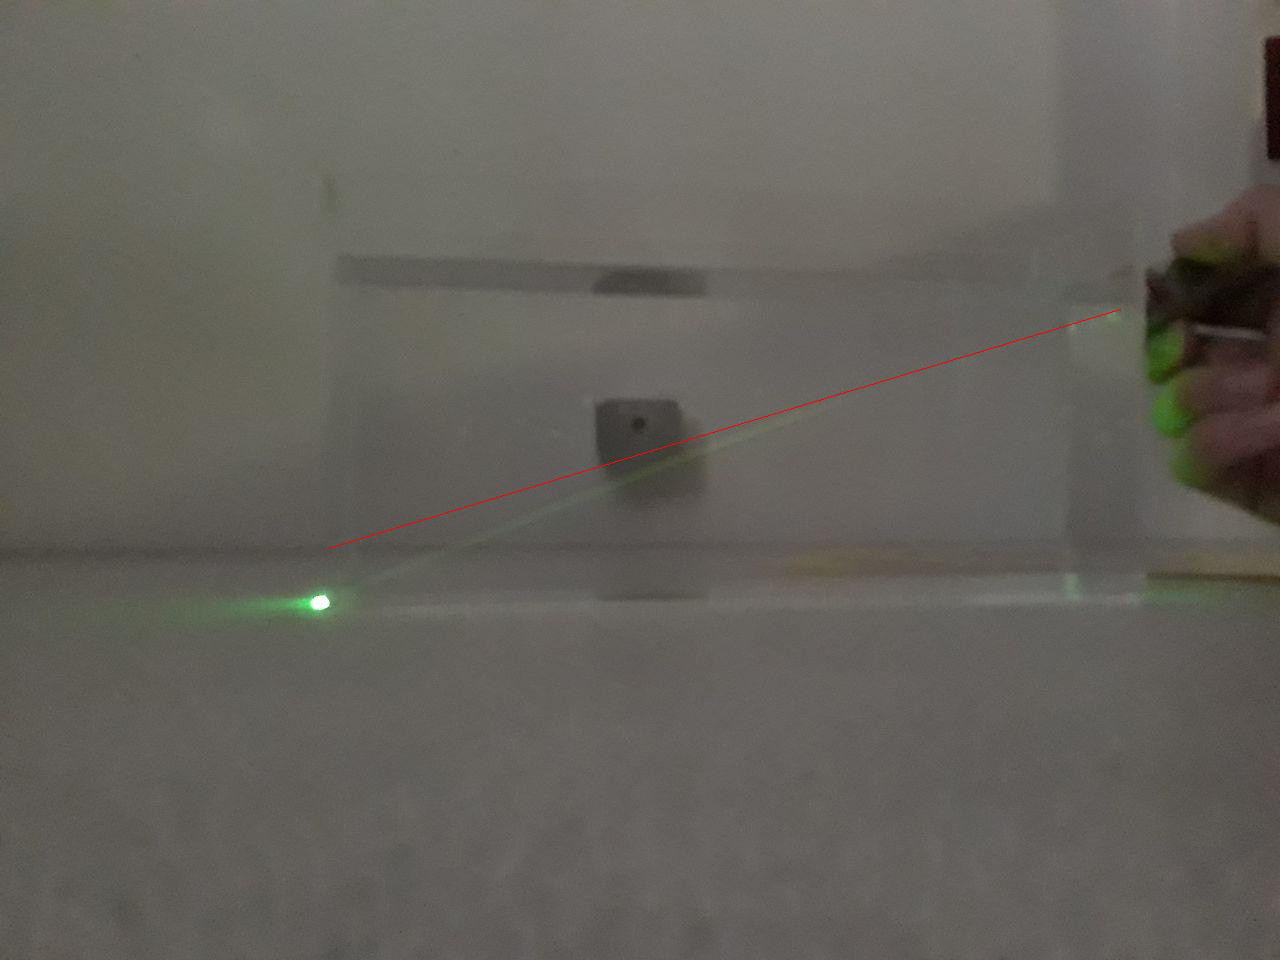
\includegraphics[width=0.7\textwidth]{Salzwasser}
		\centering
		\caption{In einen Behälter mit Salzwasser wurde schräg von der Seite mit einem grünen Laser eingestrahlt. Die rote Linie dient lediglich zur Veranschaulichung des Verlaufs, den man in einem homogenen optisch isotropen Medium erwarten würde.} 
		\label{fig_salzwasser}
		\centering
	\end{figure}
	
	\subsubsection{Prisma} %TODO Unsicherhiet ungenau weil Punkt, nur circa minimal, ungenau anfang enede
	Es wurde eine Auslenkung $a$ bei einem Abstand $d$ wie in \cref{tab_prisma} beobachtet.
	Die Unsicherheit der Auslenkung wurde mit \SI{0,14}{cm} abgeschätzt, da der Strahl orhogonal zum Lineal und auf Null justiert werden musste (ohne Prisma). 
	Zusätzlich hatte der Laserstrahl eine Durchmesser von ca. \SI{0,1}{cm}.
	Die Unsicherheit des Abstands $d$ vom Lineal zum Prisma wurde mit \SI{0,2}{cm} angenommen, da von der Mitte des Prismas zum Lineal mit dem Messraster gemessen wurde.
	\subsubsection{Brechungsindex von Wasser}
	Für den roten Laser waren die Hauptmaxima bis zur zweiten Ordnung und für den blauen bis zur dritten gut sichtbar.
	Die gemessenen Winkel sind für Luft und Wasser in \cref{tab_wasser} enthalten.
	Aufgrund der Breite des Laserstrahls nach dem Gitter wurde die Unsicherheit der analogen Winkelmessung an den Markierungen der Halbkreisküvette mit \SI{0,7}{\degree} abgeschätzt.
	Für beide Laser nehmen die Winkel ab wenn man den Behälter mit Wasser füllt, der Strahl wird also zur Flächenormalen hin gebrochen.
	\subsubsection{Brennweite der Sammellinse}
	Die Sammellinse war an ihrer Form und daran erkennbar, dass sich der Laserstrahl fokusieren lässt.
	Mit der Linse konnten Objekte vergrößert betrachtet werden, woraus auch folgt dass es sich um eine Sammellinse handelt.
	Beim Messen der Brennweite, also dem Abstand der Linse zum Fokus, ergab sich \SI{7,5}{cm} mit eine Unsicherheit von \SI{1,2}{cm}, da sich die Auflösung des Laser in diesem Bereich kaum verändert hat. 
	\subsubsection{Brennweite der Streulinse}
	Es ließ sich kein optimal kollimierter Laserstrahl, durch Variation des Abstands der Linsen, einstellen.
	Bei einem Linsenabstand von \SI{10,7 +- 1,2}{cm} änderte sich die Auflösung des Laserpunkts auf dem Schirm in verschiedenen Abständen zur Linse am geringsten.
	\subsubsection{Strahlaufweitung und Sammellinse}
	Auf den blauen Laser wurde die Strahlaufweitung montiert und so justiert, dass der Laserstrahl kollimiert ist. 
	Dieser Laserstrahl lies sich mit der Sammellinse in einen Punkt auf einem Schirm im Abstand der Brennweite bündeln.
	Wenn man nun die Linse orthogonal zum Laserstrahl verschiebt, verschiebt sich der fokussierte Punkt auf dem Schirm in die gleiche Richtung.
	Verkippt man die Linse so dass der Laserstrahl nicht mehr orthogonal auf die Linse trifft, wird der Punkt auf dem Schirm unschärfer und "verschmiert" in die Kipprichtung.

	%TODO Einflüsse von veränderten Parametern auf Messung
	\subsection{Datenanalyse}
	%TODO Berechung nach Aufgabenstellung
	\subsubsection{Brechungsindex des Prismas}
	In der Einleitung wurde \cref{eq_prisma} zur Bestimmung des Brechungsindex des Prismamaterials bei einer minimalen Ablenkung $\delta_m$ aufgeführt.
	\begin{equation}
		n = \frac{\sin\left[(\delta_m+\alpha)/2\right]}{\sin\left(\alpha/2\right)}
		\label{eq_prisma}
	\end{equation}
	\begin{equation}
		u(n) = u(\delta_m) \cdot \left|\frac{\sin(\alpha/2)\cos[(\alpha+\delta_m)/2]}{\cos(\alpha)-1}\right| %TODO a->alpha ..!
	\end{equation}

	Dabei wurde in einem Abstand $d$ eine orthogonale Auslenkung $a$ gemessen.
	Der Apexwinkel $\alpha$ beträgt $\SI{60}{\degree}$.
	Es folgt eine minimale Auslenkung $\delta_m = \arctan (a/d)$.
	Die aus den Messungen folgenden Werte sind in \cref{tab_prisma} aufgelistet.
	%TODO Laser Wellenlänge dazu?
	\begin{table}[H]
		\centering
		\begin{tabular}{ c | c | c | c | c}
			Laser & Auslenkung $a$  & Abstand $d$ & $\delta_m$ & $n$ \\ \hline
			rot & \SI{13,23 +- 0,14}{cm}&\SI{12+-0,2}{cm} & \SI{0,8341 +- 0,0098}{rad}&\SI{1,616 +- 0,006}{}\\
			blau & \SI{14,82 +- 0,14}{cm}&\SI{12+-0,2}{cm}& \SI{0,8901 +- 0,0094}{rad}&\SI{1,648 +- 0,005}{} \\
		\end{tabular}
		\caption{Aus gemessener Auslenkung des Lichtstrahls und Abstand des Lineals lässt sich der Ablenkungswinkel $\delta$ bestimmen. Der Brechungsindex des Prismas folgt widerum aus dem minimalen Ablenkungswinkel $\delta_m$.}
		\label{tab_prisma}
	\end{table}

	\subsubsection{Brechungsindex von Wasser}
	Das Snelliussche Brechungsgesetz lautet:
	\begin{equation}
		n_i \cdot \sin(\vartheta_i) = n_t \cdot \sin(\vartheta_t)
		\label{eq_snellius}
	\end{equation}
	Somit kann der Brechungsindex $n_\text{Wasser}$  mit 
	\begin{equation}
		n_\text{Wasser} = n_\text{Luft}\frac{\sin(\vartheta_\text{Luft})}{\sin(\vartheta_\text{Wasser})}
	\end{equation}
	\begin{equation}
		u(n_\text{Wasser}) = n_\text{Luft} \sqrt{\left(\frac{\cos(\vartheta_\text{Luft})}{\sin(\vartheta_\text{Wasser})} u(\vartheta_\text{Luft})\right)^2 + \left(\frac{\sin(\vartheta_\text{Luft})\cos( \vartheta_\text{Wasser})}{\sin(\vartheta_\text{Wasser})^2}u(\vartheta_\text{Wasser})\right)^2}
	\end{equation}

	bestimmt werden.
	Die Messwerte sowie resultierende Brechungsindizes sind in \cref{tab_wasser} aufgeführt.
	Gemittelt ergibt sich ein Brechungsindex für Wasser bei rotem Licht von \SI{1,309 +- 0,010}{} und bei blauem \SI{1,318 +- 0,012}{}.
	%TODO Laser Wellenlänge dazu?
	\begin{table}[H] %TODO was hast du für n_Luft benutzt?
		\centering
		\begin{tabular}{ c | c | c | c | c}
			Laser & Maximum Ordnung & $\vartheta_\text{Luft}$ & $\vartheta_\text{Wasser}$ & $n_\text{Wasser}$ \\ \hline
			rot & -2 &\SI{52,8 +- 0,3}{\degree} & \SI{37,5 +-0,3}{\degree} & \SI{1,308 +- 0,010}{}\\
			& -1 &\SI{23,8 +- 0,3}{\degree} & \SI{18+-0,3}{\degree} & \SI{1,306 +- 0,026}{}\\
			& 1 &\SI{24 +- 0,3}{\degree} & \SI{18+-0,3}{\degree} & \SI{1,316 +- 0,026}{}\\
			& 2 &\SI{53,5 +- 0,3}{\degree} & \SI{38+-0,3}{\degree} & \SI{1,306 +- 0,010}{}\\ \hline
			blau & -3 & \SI{48,0 +- 0,3}{\degree}&\SI{34,5+-0,3}{\degree}& \SI{1,312 +- 0,012}{} \\
			& -2 & \SI{30,0 +- 0,3}{\degree}&\SI{22,2+-0,3}{\degree}& \SI{1,323 +- 0,021}{} \\
			& -1 & \SI{14,5 +- 0,3}{\degree}&\SI{10,9+-0,3}{\degree}& \SI{1,324 +- 0,045}{} \\
			& 1 & \SI{14,5 +- 0,3}{\degree}&\SI{11+-0,3}{\degree}& \SI{1,312 +- 0,044}{} \\
			& 2 & \SI{30,0 +- 0,3}{\degree}&\SI{22,2+-0,3}{\degree}& \SI{1,323 +- 0,021}{} \\
			& 3 & \SI{48,5 +- 0,3}{\degree}&\SI{34,8+-0,3}{\degree}& \SI{1,312 +- 0,012}{} \\

		\end{tabular}
		\caption{Für einen roten und einen roten Laser sind die Winkel Beugungsmaxim,a die durch ein Gitter erzeugt werden, aufgeführt. Unmittelbar hinter dem Gitter befand sich eine einmal mit Luft und einmal mit destilliertem Wasser gefüllte Halbkreisküvette. Aus der Winkeländerung lassen sich die Brechungsindizes von Wasser nach dem Snelliusschen Brechungsgesetz bestimmen.} 
		\label{tab_wasser}
	\end{table}
	
	\subsubsection{Brennweite Streulinse}
	In der Einführung wurde die Brennweite eines Linsensystems mit folgender Formel beschrieben:
	\begin{equation}
		\frac{1}{f} = \frac{1}{f_1} + \frac{1}{f_2} - \frac{d}{f_1 f_2}
		\label{eq_linsensystem}
	\end{equation}
	Im Falle eines eintreffenden kollimierten Strahls, der nach dem Linsensystem erneut kollimiert ist, liegt der Fokus im Unendlichen.
	Der Kehrwert $1/f$ nähert sich also Null an.
	Mit \cref{eq_linsensystem} folgt daraus, dass $d = f_1 + f_2$ gelten muss.
	Die Brennweite der Sammellinse beträgt \SI{7,5+-1,2}{cm} und der Abstand der Linsen $d$ war \SI{10,7 +- 1,2}{cm}.
	Es ergibt sich also eine Brennweite von \SI{3,2+-1,7}{cm} für die Streulinse.
	\subsection{Diskussion}
	%TODO Bezug/Nutzten oder sonst was
	%TODO auch hier die Hypothese wiederholen
	%TODO keine Messwerte hier, nach manchen Menschen, zumindest "direkt" erstellte Diagramme net hier, auch wenn Lesbarkeit-bla
	\subsubsection{Demonstrationsversuch}
	Der gekrümmte Verlauf des Laserstrahls kommt dadurch zustande, dass durch die Erdanziehungskraft die Konzentration des Salzes im Gefäß von oben nach unten zunimmt.
	Der Brechungsindex nimmt mit der Konzentration und somit ebenfalls von oben nach unten zu. %TODO true?
	Demnach trifft der Laser auf unendlich viele Grenzflächen aus zwei Materialien mit minimal unterschiedlichem Brechungsindex.
	Deshalb wird er an jeder dieser Grenzflächen etwas mehr gebrochen und insgesamt sieht man einen gekrümmten Verlauf.
	\subsubsection{Prisma aus Flintglas}
	Es entstehen mehrere Strahlen nach dem Prisma, da sowohl beim Eintritt in als auch beim Austritt aus dem Prisma immer nur ein Teil des Laserstrahls transmittiert wird.
	Die Strahlen abseits des Strahls, der sich durch zweifache Transmission ergibt, entstehen also durch eine Kombination aus Transmissionen und Reflexionen.
	Der Strahl durch zweifache Transmission verhielt sich wie auf Basis der Einführung erwartet und bildete einen minimalen Ablenkungswinkel, von dem ein Drehen des Prismas in beide Richtungen zu einer erhöhten Ablenkung führte. %TODO ist bissl auch Beobachtung
	
	Die Literatur gibt für den Brechungsindex von Flintglas einen Wert von \SI{1,613}{} an \cite{flintglasref}.
	Da hier nicht eindeutig ist, wo im sichtbaren Spektrum dieser Wert gemessen wurde, kann er zwar nicht die Messwerte bezogen auf ihre präzise Wellenlänge bestätigen, aber da er innerhalb der Unsicherheiten des gemessenen Brechungsindexes bei rotem Laser (\SI{1,616 \pm 0,006}{}) liegt, kann der Literaturwert für den Bereich des roten Lichts bestätigt werden.
	Außerdem kann die Vermutung, dass der Brechungsindex bei rotem Licht leicht kleiner als bei blauem ist, mit hinreichender Signifikanz bestätigt werden (vgl. \cref{tab_prisma}).
	
	\subsubsection{Brechungsindex von Wasser}
	Für Wasser gibt die Literatur einen Brechungsindex von \SI{1,333}{} an \cite{flintglasref}.
	Dies liegt innerhalb der 1,3-fachen Unsicherheit des Mittelwerts für blaues Licht.
	Dies ist ausreichend, um den Literaturwert für einen Bereich des sichtbaren Lichts zu bestätigen.
	Dass der Brechungsindex mit steigender Wellenlänge sinkt, entspricht zwar den Messwerten von \SI{1,309\pm 0,01}{} bei rotem Licht und \SI{1,318}{} bei blauem, aber die Signifikanz ist hier aufgrund der geringen Differenz dieser Werte im Vergleich zu ihren Fehlern sehr gering.
	
	\subsubsection{Linsen}
	
	%TODO linsen
	%TODO Astigmatismus ist bei Strahlaufweitung und Verkippung der Sammellinse aufgetreten
	%TODO Keine messbare sphärische Aberration beim Verschieben der Linse aufgetreten
	%TODO Chromatische Aberration bei Wasser Experimenten, kann gut sein dass du des aber schon hast, lel
	
	Es wurde erwartet, dass eine der Linsen eine Streu- und die andere eine Sammellinse ist, was bedeuten würde, dass die Brennweite der einen Linse positiv und die der anderen negativ ist.
	Dies konnte nicht nachgewiesen werden, da beide Brennweiten positiv waren.
	Dies hängt vermutlich damit zusammen, dass die Messung so unpräzise war, dass der Messwert der Brennweite der hypothetischen Streulinse um weniger als den doppelten Fehler von Null verschieden ist.
	\section{Schlussfolgerung}
	%TODO Rückgriff auf Hypothese und drittes Nennen dieser
	Es ließen sich verschiedene optische Komponenten untersuchen und die Brechungsindizes von blauem und rotem Licht von Wasser und Flintglas bestimmen.
	Die gemessenen Brechungsindizes von Flintglas bei blauem und roten Licht konnten den Literaturwert und die Hypothese des mit der Wellenlänge abnehmenden Brechungsindex bestätigen.
	Auch für Wasser konnte der Literaturwert bestätigt werden.
	Die oben genannte Beziehung zwischen Brechungsindex und Wellenlänge konnte jedoch aufgrund des nicht hinreichend präzisen Versuchsaufbaus nicht bestätigt werden.
	Eine präzisere Messung würde einen Laser mit geringerem Strahldurchmesser und eine genauere Skala auf der Halbkreisküvette sowie einen besser abgedunkelten Raum voraussetzen. %TODO geringerer Strahldurchmesser => fokussierteren Laser? ist das besser?
	Die Untersuchung der Linsen konnte die Hypothese, dass eine der Linsen eine Streu- und die andere eine Sammellinse ist, nicht bestätigen.
	Für eine erfolgreichere Untersuchung wäre hier eine optische Bank, die sicherstellt, dass Linsen und Laser in einer Linie stehen hilfreich gewesen.
	Außerdem hätte die Durchführung mit einem aufgeweiteten Strahl es deutlich vereinfacht, festzustellen, ob der Strahl kollimiert ist.
	%TODO Quellen zitieren, Websiten mit Zugriffsdatum
	%TODO Verweise auf das Laborbuch (sind erlaubt)
	%TODO Tabelle + Bilder mit Beschriftung
	\printbibliography
\end{document}
